Был доработан плагин <<SearchProgram>> (рис.~\ref{kucher_1:kucher_1}). Теперь при подаче образа с операционной системой не нужно указывать, какая ОС (Windows XP/7/8/8.1) на образе. Он использует написанный ранее плагин DetectKernel32Win, который определяет ОС. В итоге, плагин <<SearchProgram>> не требует каких-либо действий от пользователя.

В течение семестра <<gitlab>> был перенесен на другой домен, поэтому надо было исправить скрипты <<COEX>>, чтобы они работали с новым доменом (текущее задание --- рис.~\ref{kucher_2:kucher_2}). Скрипты clone.sh и test.sh были исправлены (рис.~\ref{kucher_3:kucher_3}).

\begin{figure}[h!]
\center{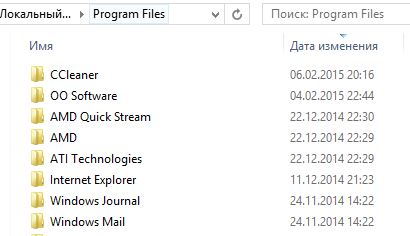
\includegraphics[width=0.5\linewidth]{kucher_1}}
\caption{ Блок-схема плагина <<SearchProgram>> }
\label{kucher_1:kucher_1}
\end{figure}

\begin{figure}[h!]
\center{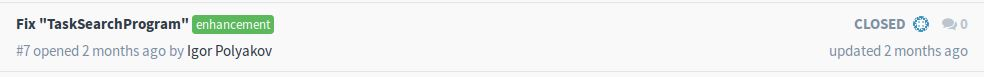
\includegraphics[width=0.8\linewidth]{kucher_2}}
\caption{ Закрытый issue <<Fix TaskSearchProgram>> }
\label{kucher_2:kucher_2}
\end{figure}
	
\begin{figure}[h!]
\center{
\includegraphics[width=0.8\linewidth]{kucher_3}}
\caption{ Закрытый issue <<Исправить скрипты clone & test>> }
\label{kucher_3:kucher_3}
\end{figure}
	
\clearpage 
\subsection{Создание репозитория проекта <<COEX>>}

В текущем семестре была поставлена задача создать репозиторий для хранения deb-пакетов <<COEX>>.
Репозиторий разворачивался на виртуальной машине с ОС Debian 7.9. Для создания репозитория была выбрана программа <<reprepro>>.
Reprepro является инструментом для управления APT репозиториев. Он в состоянии управлять многократными репозиториями для многократных версий распределения и одного пула пакета. Reprepro может обработать обновления из входящего каталога, пакет копии (ссылки) между версиями распределения, перечислить все пакеты и/или версии пакета, доступные в репозитории и т.д. 
Reprepro поддерживает внутреннюю базу данных (.DBM файл) содержания репозитория, который делает его довольно быстрым и эффективным.
В добавок, в Reprepro есть возможность подтверждения подлинности пакетов с помощью GPG – ключа.
GNU Privacy Guard (GnuPG, GPG) — свободная программа для шифрования информации и создания электронных цифровых подписей. С помощью нее генерируем GPG – ключ.
В качестве веб – сервера был выбран «Nginx», т.к. легко масштабируется на минимальном железе.
Установка программы reprepro выполняется следующей командой: aptitude install reprepro. Далее, создаем каталог <<repository>> в /var/www/. Для настройки репозитория необходимо создать два конфигурационных файла <<distributions>> и <<options>> в папке <<repository>>.~\cite{anosov} 

Настроенный конфигурационный файл <<distributions>> программы <<reprepro>> выглядит следующим образом (рис.~\ref{kucher_4:kucher_4}):

\begin{figure}[h!]
\center{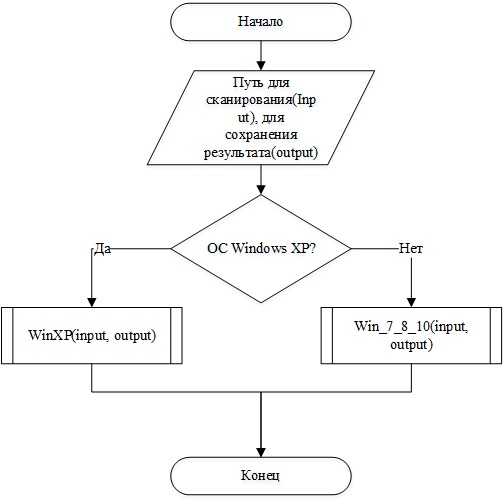
\includegraphics[width=0.6\linewidth]{kucher_4}}
\caption{ Конфигурационный файл <<distributions>> }
\label{kucher_4:kucher_4}
\end{figure}

Параметр <<SignWith: yes>> указывает на то, что репозиторий будет использовать GPG – ключ для подтверждения подлинности пакетов.

Настроенный конфигурационный файл <<options>> (рис.~\ref{kucher_5:kucher_5}):
	
\begin{figure}[h!]
\center{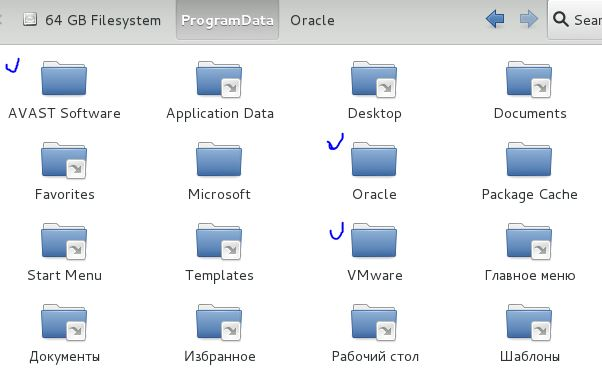
\includegraphics[width=0.6\linewidth]{kucher_5}}
\caption{ Конфигурационный файл <<options>> }
\label{kucher_5:kucher_5}
\end{figure}
	
<<Verbose>> определяет, что всегда будет выводиться информация о ходе выполнения команды, а <<ask-passphrase>> заставляет <<reprepro>> спрашивать пароль для GPG-ключа при добавлении нового deb-пакета в репозиторий.
Генерация GPG-ключа выполняется командой gpg --gen-key.

Для добавлении файлов в репозиторий используется следующая команда (при условии, что находимся в директории <<repository>>): reprepro –b . includedeb linux /путь к deb-пакету.

После выполнения этих действий настройка репозитория закончена. Он доступен локально. Следует настроить веб-сервер, чтобы предоставить доступ к репозиторию через интернет. Также был зарегистрирован домен repa.coex.su для репозитория проекта. Настроенный конфигурационный файл для веб-сервера <<Nginx>> выглядит следующим образом (рис.~\ref{kucher_6:kucher_6}):
	
\begin{figure}[h!]
\center{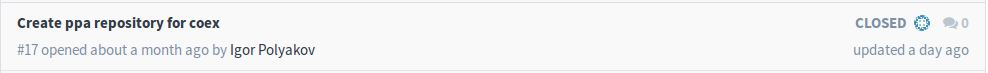
\includegraphics[width=0.6\linewidth]{kucher_6}}
\caption{ Конфигурационный файл <<repa.coex.su>> веб-сервера <<Nginx>> }
\label{kucher_6:kucher_6}
\end{figure}
	
Так как созданный репозиторий --- публичный, то нужно ограничить доступ к каталогам /conf и /db, содержащим сведения о настройках репозитория. Демонстрация веб-страниц сайта представлена на рисунках~\ref{kucher_7:kucher_7},~\ref{kucher_8:kucher_8},~\ref{kucher_9:kucher_9}.  
	
\begin{figure}[h!]
\center{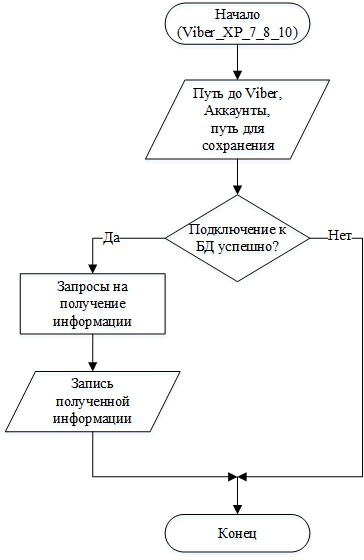
\includegraphics[width=0.6\linewidth]{kucher_7}}
\caption{ Демонстрация страницы repa.coex.su }
\label{kucher_7:kucher_7}
\end{figure}
	
\begin{figure}[h!]
\center{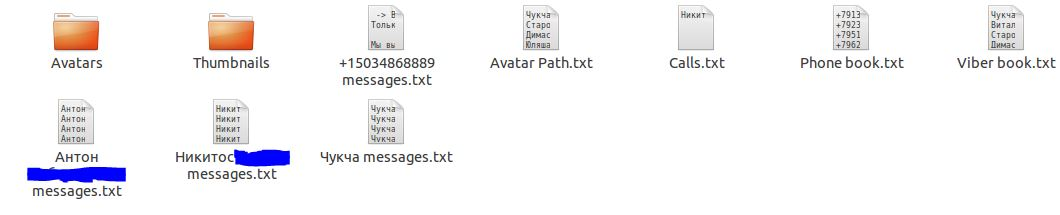
\includegraphics[width=0.6\linewidth]{kucher_8}}
\caption{ Демонстрация страницы repa.coex.su/conf/ }
\label{kucher_8:kucher_8}
\end{figure}
	
\begin{figure}[h!]
\center{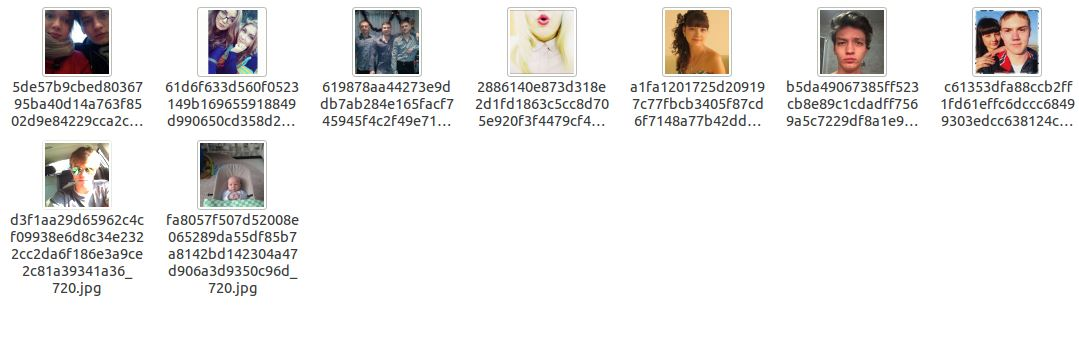
\includegraphics[width=0.6\linewidth]{kucher_9}}
\caption{ Демонстрация страницы repa.coex.su/db/ }
\label{kucher_9:kucher_9}
\end{figure}
	
	
Нужно было предоставить пользователям репозитория возможность свободно получать открытый GPG – ключ. Для этого было принято решение воспользоваться публичным GPG – сервером http://keyserver.ubuntu.com. Но этот GPG – сервер принимает ключи в формате ASCII – armored. Поэтому сначало следует конвертировать файл pubring.gpg в pubring.asc следующей командой: gpg –output pubring.asc –export –a \$GPGKEY. Полученный файл загружаем на публичный GPG – сервер.~\cite{nixp} 

Теперь пользователям репозитория нужно установить открытый GPG – ключ репозитория repa.coex.su командами: gpg --keyserver keyserver.ubuntu.com --recv <<номер ключа, который запросит репозиторий>> и gpg --export --armor <<номер ключа, который запросит репозиторий>> | apt-key add.

После успешного экспорта нужно добавить строчку deb http://repa.coex.su linux non-free в файл /etc/apt/sources.list.

Обновить список пакетов командой aptitude update и установить <<COEX>> командой aptitude install coex. Задача создания репозитория проекта выполнена успешно, о чем свидетельствует закрытый <<issue>> (рис.~\ref{kucher_10:kucher_10}).
	
\begin{figure}[h!]
\center{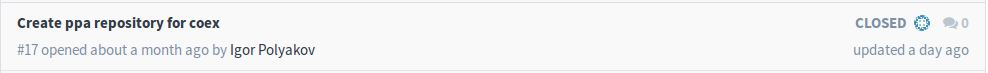
\includegraphics[width=0.8\linewidth]{kucher_10}}
\caption{ Закрытый issue <<Create ppa repository for coex>> }
\label{kucher_10:kucher_10}
\end{figure}


\clearpage






